\documentclass{beamer}
\usepackage{ctex, hyperref}
\usepackage[T1]{fontenc}

\usepackage{latexsym,amsmath,multicol,booktabs,calligra, mathtools}
\usepackage{graphicx,pstricks,listings,stackengine}
\usepackage{xspace, array}
\usepackage[dvipsnames]{xcolor}
\usepackage{pifont, stmaryrd}
\usepackage{mathpartir} % \inferrule and mathpar env.
\usepackage{dashrule} % advanced hlines
\usepackage{subcaption}
\usepackage{tabularray}
\usepackage{rotating}


\usepackage{tikz}
\usepackage{pgfplots}
% \usetikzlibrary{arrows.meta, positioning, fit, external}
\usetikzlibrary{arrows.meta, positioning, fit, calc}

% Execution Graph & Declarative Semantics
\tikzset{
    executiongraph/.style={
        >=Stealth,
        node distance=1.2cm and 1.5cm
    },
    % Node styles
    persisted/.style={
        draw=none, 
        fill=hlcolor, 
        rounded corners=2pt,
        inner sep=3pt,
        font=\sffamily
    },
    visible/.style={
        font=\sffamily
    },
    invisible/.style={
        font=\sffamily,
        text=gray
    },
    % Bounding Box
    failed/.style={
        draw=BlueViolet,
        line width=0.8pt,
        rounded corners=2pt,
        dashed,
        inner sep=6pt
    },
    % Arrow styles
    solidarrow/.style={->, shorten >=2pt, shorten <=2pt},
    rfarrow/.style={->, shorten >=2pt, shorten <=2pt, color=teal, dashed},
    tpoarrow/.style={->, dotted, color=red, line width=1pt, shorten >=2pt, shorten <=2pt},
    moarrow/.style={->, dotted, color=orange, line width=1pt, shorten >=2pt, shorten <=2pt},
    % dtpoarrow/.style={->, dotted, color=purple!80!black, line width=1pt, shorten >=2pt, shorten <=2pt}
}

\author{韩志磊}
\title{并发系统的崩溃语义及其形式化验证技术}
% \subtitle{最终学术报告}
\institute{清华大学软件学院}
\date{\today}
\usepackage{Tsinghua}

% defs
\def\cmd#1{\texttt{\color{red}\footnotesize $\backslash$#1}}
\def\env#1{\texttt{\color{blue}\footnotesize #1}}
\definecolor{deepblue}{rgb}{0,0,0.5}
\definecolor{deepred}{rgb}{0.6,0,0}
\definecolor{deepgreen}{rgb}{0,0.5,0}
\definecolor{halfgray}{gray}{0.55}

\lstset{
    basicstyle=\ttfamily\small,
    keywordstyle=\bfseries\color{deepblue},
    emphstyle=\ttfamily\color{deepred},    % Custom highlighting style
    stringstyle=\color{deepgreen},
    numbers=left,
    numberstyle=\small\color{halfgray},
    rulesepcolor=\color{red!20!green!20!blue!20},
    frame=shadowbox,
}

\newcommand{\highlight}[1]{{\color{tsinghua}#1}}

% Other Functions & Operators
\newcommand{\obs}{\ensuremath\mathit{obs}\xspace}
\newcommand{\domain}{\ensuremath\mathit{dom}\xspace}
\newcommand{\codomain}{\ensuremath\mathit{codom}\xspace}
\newcommand{\add}{\ensuremath\mathtt{Add}\xspace}
\newcommand{\assigns}{\ensuremath{\coloneq}\xspace}
\newcommand{\node}{\ensuremath\mathtt{node}\xspace}
\newcommand{\owner}{\ensuremath\mathtt{owner}\xspace}
\newcommand{\region}{\ensuremath\mathtt{region}\xspace}
\newcommand{\volatile}{\ensuremath\mathtt{volatile}\xspace}
\newcommand{\traces}{\ensuremath\mathcal{T}\xspace}
\newcommand{\tp}{\ensuremath\mathit{tp}\xspace}            

\newcommand{\cmark}{\ding{51}}
\newcommand{\xmark}{\ding{55}}

% Types & Sets
\newcommand{\threadset}{\ensuremath{\mathcal{T}}\xspace}
\newcommand{\nodeset}{\ensuremath{\mathcal{N}}\xspace}
\newcommand{\pnodeset}{\ensuremath{\mathcal{N}_P}\xspace}
\newcommand{\mnodeset}{\ensuremath{\mathcal{N}_M}\xspace}
\newcommand{\initset}{\ensuremath{\mathtt{I}}\xspace}
\newcommand{\labelset}{\ensuremath\operatorname{Lab}\xspace}
\newcommand{\plabel}{\ensuremath{\operatorname{PLab}}\xspace}
\newcommand{\variables}{\ensuremath{\mathcal{L}}\xspace}
\newcommand{\values}{\ensuremath{\mathcal{V}}\xspace}
\newcommand{\registers}{\ensuremath{\mathcal{R}}\xspace}
\newcommand{\sbuffer}{\ensuremath{\mathsc{SBuffer}}\xspace}
\newcommand{\pbuffer}{\ensuremath{\mathsc{PBuffer}}\xspace}
\newcommand{\cache}{\ensuremath{\mathsc{Cache}}\xspace}
\newcommand{\memory}{\ensuremath{\mathsc{Mem}}\xspace}
\newcommand{\eventset}{\ensuremath{\mathcal{E}}\xspace}
\newcommand{\egraph}{\ensuremath\mathsc{EGraph}\xspace}

% 定义并发程序环境: concurrentcode
\newenvironment{concurrentcode}
{
    \begin{center}
    \renewcommand{\arraystretch}{1.1} % 稍微拉开行间距
    \ttfamily                         % 全局切换为等宽字体
    \begin{tabular}{>{\raggedright\arraybackslash}l || >{\raggedright\arraybackslash}l}
}
{
    \end{tabular}
    \end{center}
}

\newcommand{\expected}[1]{\color{Purple}#1\color{black}}

\newenvironment{concurrentcode3}
{
    \begin{center}
    \renewcommand{\arraystretch}{1.1} 
    \ttfamily                         
    \begin{tabular}{>{\raggedright\arraybackslash}l || >{\raggedright\arraybackslash}l || >{\raggedright\arraybackslash}l}
}
{
    \end{tabular}
    \end{center}
}


\begin{document}

\kaishu
\begin{frame}
    \titlepage
    \begin{figure}[htpb]
        \begin{center}
            \includegraphics[width=0.2\linewidth]{pic/Tsinghua_University_Logo.eps}
        \end{center}
    \end{figure}
\end{frame}

\begin{frame}
    \tableofcontents[sectionstyle=show,subsectionstyle=show/shaded/hide,subsubsectionstyle=show/shaded/hide]
\end{frame}


\section{课题背景}

\begin{frame}{内存模型}
    随着计算系统不断发展，程序语义随之变化，从而要求新的语义建模工具。
    % 存与算是计算系统发展的两个维度，也对应着形式化语义模型的发展脉络。形式
    \begin{itemize}
        \item 算（经典形式语义学）：规定与平台无关的程序执行语义
        \item 存（\highlight{内存模型}）：刻画访存操作的顺序与语义
    \end{itemize}
    \vspace{0.5em}
    \centering
    \begin{tikzpicture}[x=1cm,y=1cm]
        \draw[very thick, gray!70, -{Latex[length=2mm]}] (0,0) -- (11.2,0);

        \foreach \x/\idx in {1.4/1,5.6/2,9.8/3} {
            \only<\idx->{
                \fill[tsinghua] (\x,0) circle (2.5pt);
            }
        }

        \only<1->{\node[above=0.6cm] at (1.4,0) {\includegraphics[width=1.7cm]{pic/Tsinghua_University_Logo.eps}};}
        \only<2->{\node[above=0.6cm] at (5.6,0) {\includegraphics[width=1.7cm]{pic/Tsinghua_University_Logo.eps}};}
        \only<3->{\node[above=0.6cm] at (9.8,0) {\includegraphics[width=1.7cm]{pic/Tsinghua_University_Logo.eps}};}

        \only<1->{\node[below=0.35cm] at (1.4,0) {串行};}
        \only<2->{\node[below=0.35cm] at (5.6,0) {顺序一致性};}
        \only<3->{\node[below=0.35cm] at (9.8,0) {弱内存模型};}
        \only<1->{\node[below=0.9cm] at (1.4,0) {1940s $\sim$ 1960s};}
        \only<2->{\node[below=0.9cm] at (5.6,0) {1979};}
        \only<3->{\node[below=0.9cm] at (9.8,0) {1990s $\sim$ 2010s};}
    \end{tikzpicture}
\end{frame}

\begin{frame}{新兴并发系统}
    \begin{minipage}[c]{0.6\linewidth}
        \begin{figure}
            \centering
            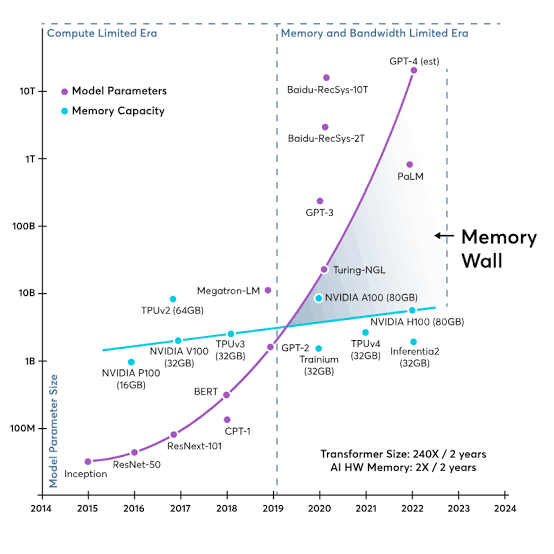
\includegraphics[width=\linewidth]{pic/memory-wall.png}
        \end{figure}
    \end{minipage}
    \hfill
    \begin{minipage}[c]{0.35\linewidth}
        本课题研究近年涌现出的一批新兴并发系统，探索其语义建模与验证技术。
        \begin{itemize}
            \item 安全攸关系统的数据安全$\rightarrow$非易失性内存系统
            \item 内存墙问题$\rightarrow$分离式共享内存系统
        \end{itemize}
    \end{minipage}
\end{frame}

\begin{frame}{研究对象}
    新兴并发系统中的\highlight{崩溃}会影响程序执行，而在传统的内存模型框架中并未考虑崩溃这一维度。

    \vfill
    \centering
    \small
    \renewcommand{\arraystretch}{1.2}
    \begin{tabular}{ccc}
    	传统多线程并发程序 & 非易失性内存系统 & 分离式共享内存系统 \\
    	\includegraphics[width=0.14\textwidth]{pic/Tsinghua_University_Logo.eps}
    	    & \includegraphics[width=0.14\textwidth]{pic/Tsinghua_University_Logo.eps}
    	    & \includegraphics[width=0.14\textwidth]{pic/Tsinghua_University_Logo.eps} \\
    	单机        & 单机       & 分布式       \\
    	DRAM      & NVMM     & DSM       \\
    	---       & 2019（傲腾） & 2023（CXL） \\
    	无崩溃模型     & 完全崩溃模型   & 部分崩溃模型    \\
    \end{tabular}
\end{frame}

\begin{frame}{研究思路}
    \centering
    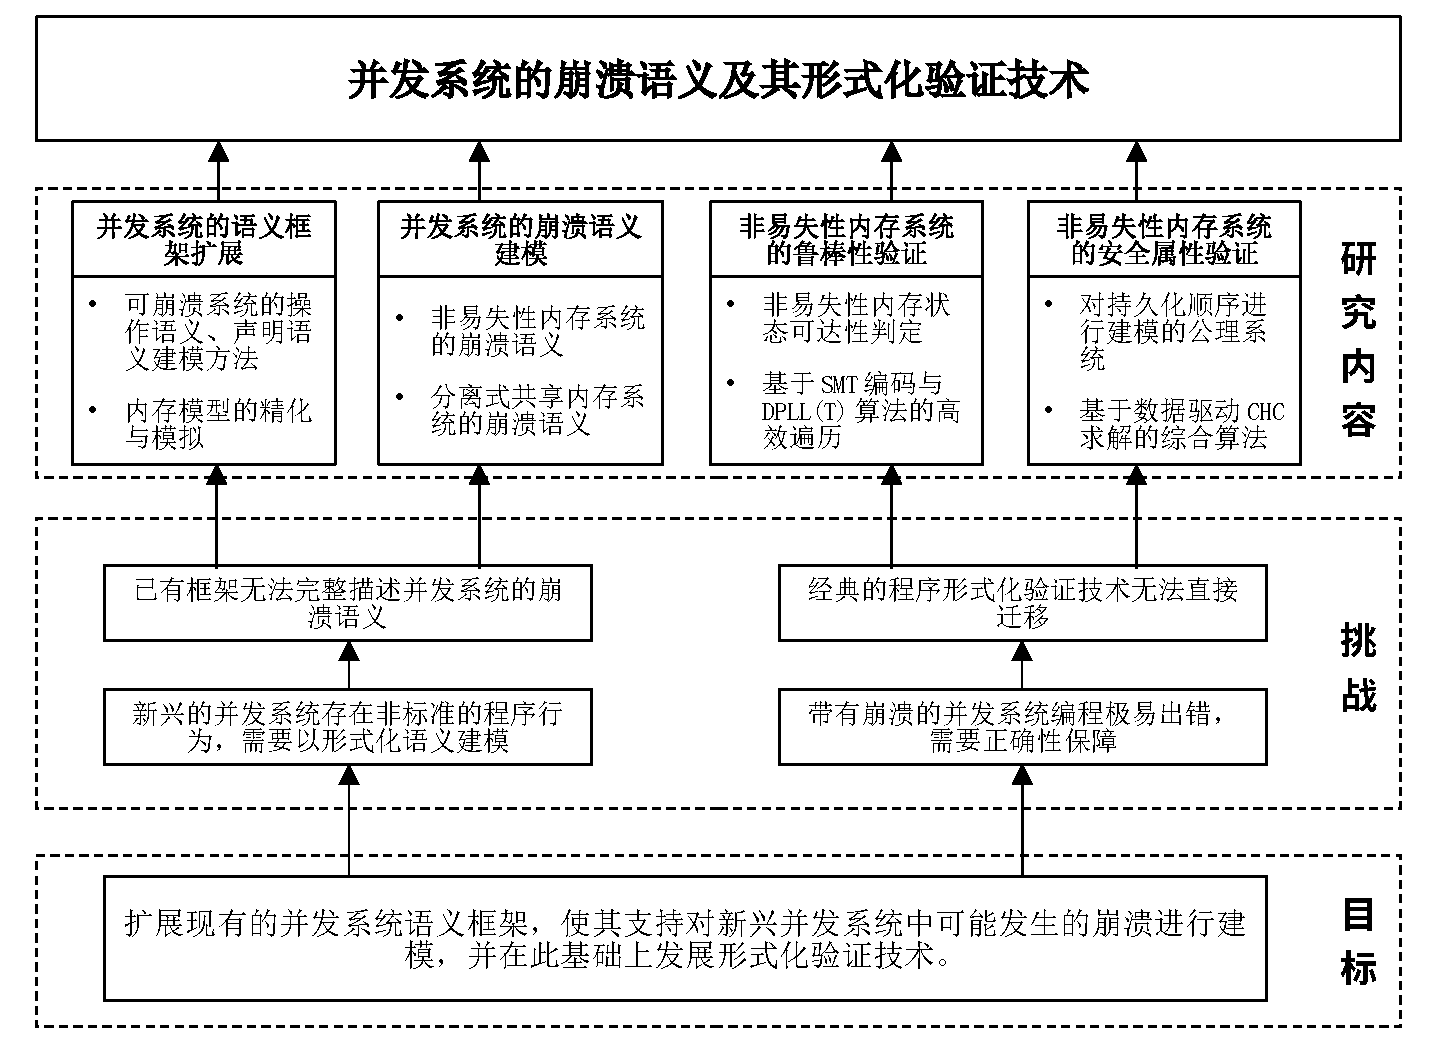
\includegraphics[width=0.9\linewidth]{pic/methodology.pdf}
\end{frame}

\section{崩溃语义}

\begin{frame}{示例}
    \centering
    \begin{columns}
        \begin{column}{0.4\textwidth}
            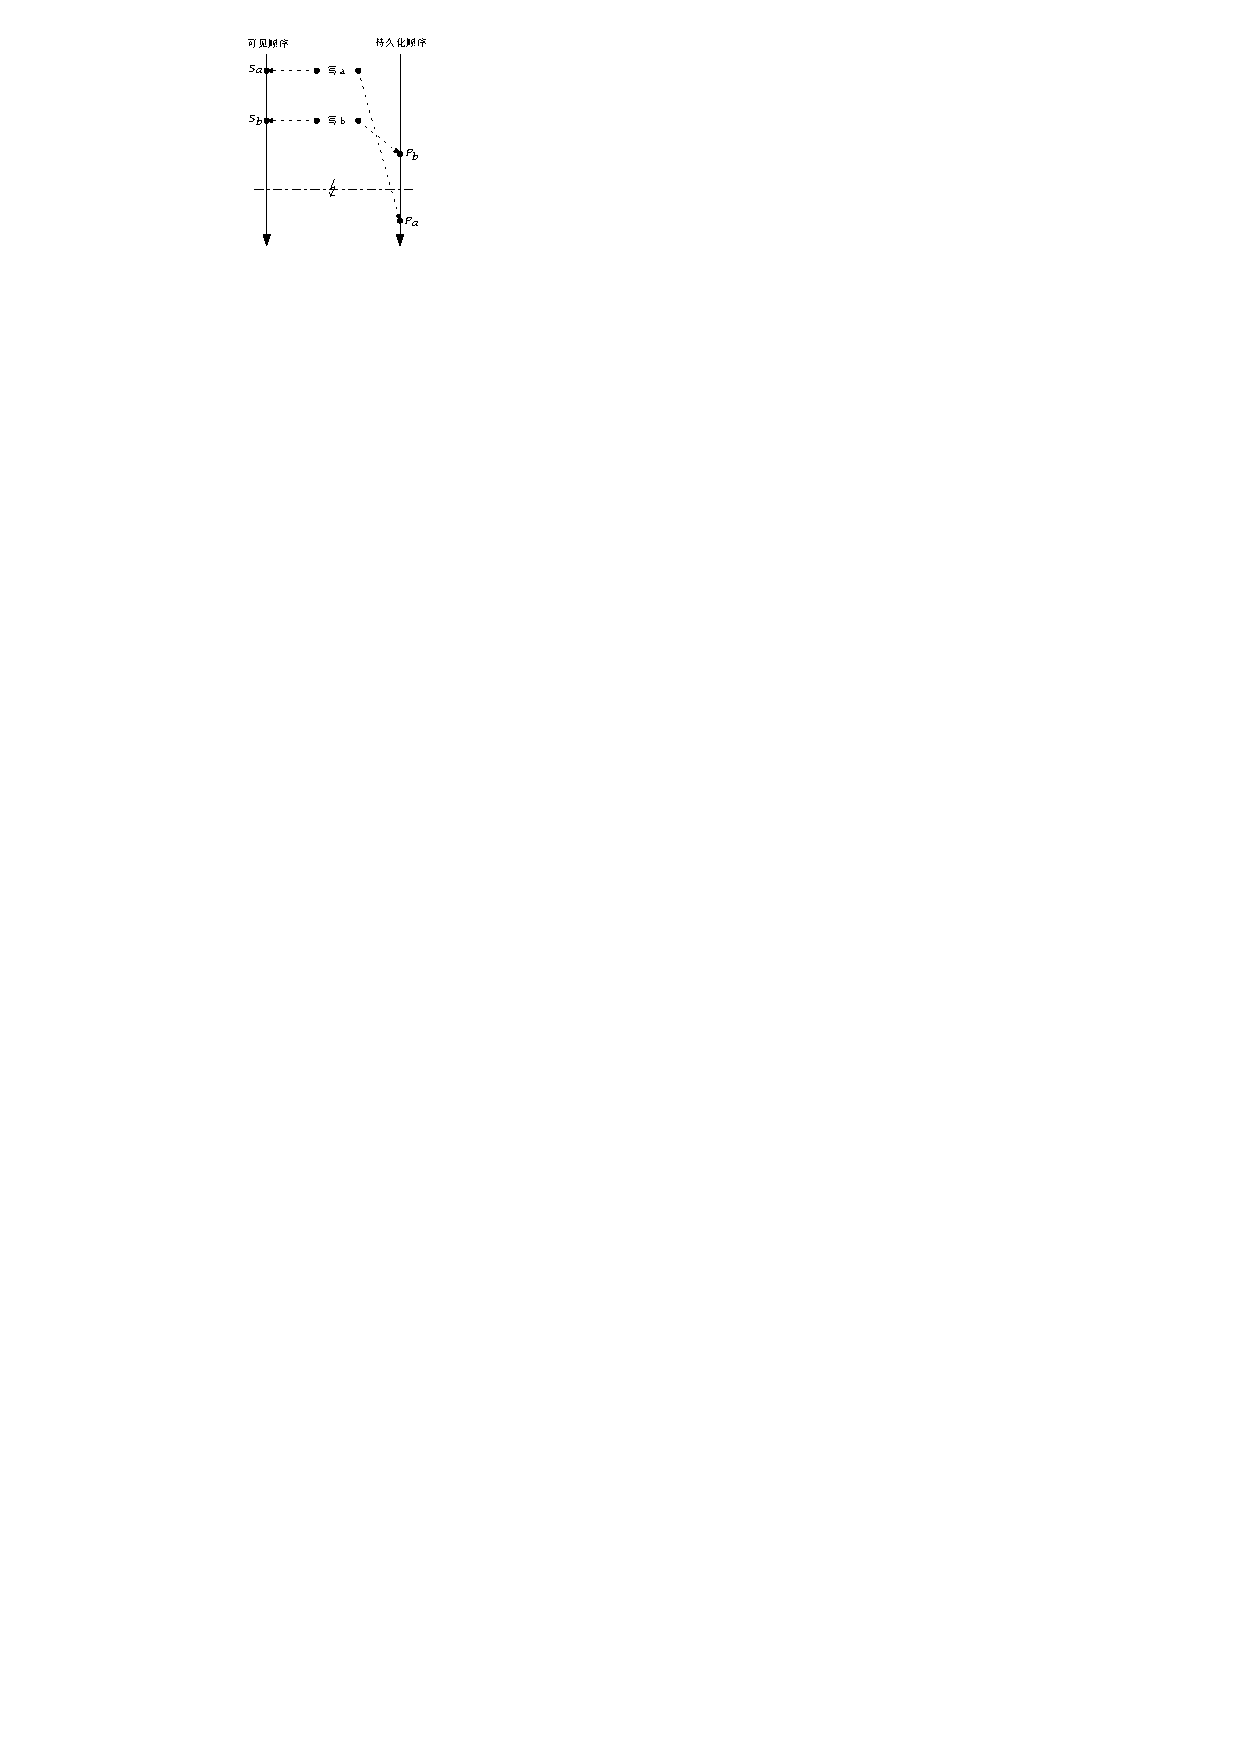
\includegraphics[width=\linewidth]{pic/nvm-intro-exp.pdf}
        \end{column}

        \begin{column}{0.4\textwidth}
            在NVMM下，程序$a \assigns 1; b \assigns 1$的一条可能执行：
            \begin{itemize}
                \item $a \assigns 1$ 先于 $b \assigns 1$ 被处理器发射
                \item $b \assigns 1$ 先于 $a \assigns 1$ 到达主存
                \item 假设在$a \assigns 1$ 到达主存前发生崩溃，观察到状态$a \mapsto 0, b \mapsto 1$
            \end{itemize}
        \end{column}
    \end{columns}
    
    \vfill
    如何刻画上述程序行为？
\end{frame}

\begin{frame}{示例2}
	\begin{concurrentcode}
		x \assigns 1; & a \assigns x; \expected{// 1}               \\
		& b \assigns x; \expected{// 0}                  \\
	\end{concurrentcode}

    \begin{itemize}
        \item x86/TSO: 不合法
        \item NVMM: 不合法
        \item DSM: 合法
    \end{itemize}

    \vfill
    \centering
    如何刻画上述程序行为？
\end{frame}

\begin{frame}{内存层级}
    \centering
    NVMM 可被视为 DSM 在单机上的特例

    \begin{columns}
        \begin{column}{0.34\textwidth}
            \begin{figure}
                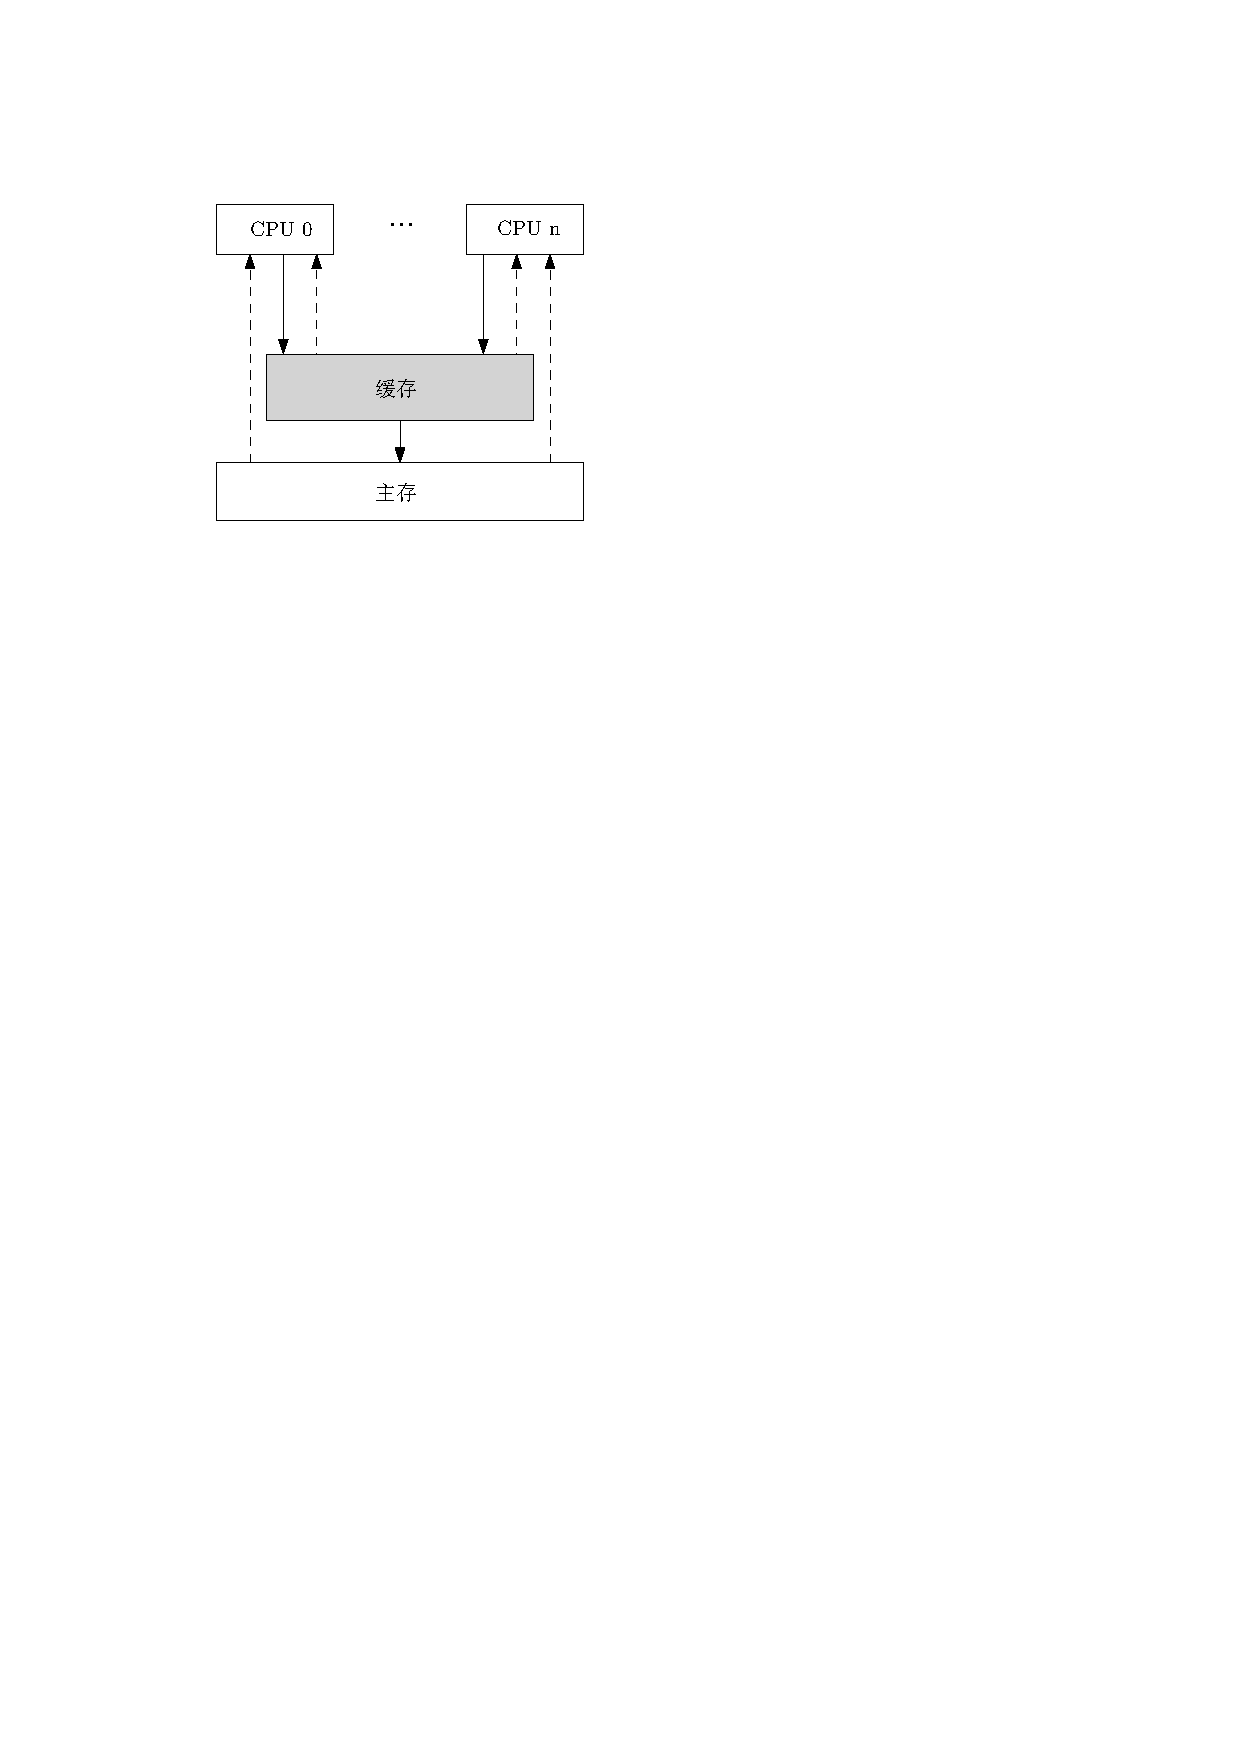
\includegraphics[width=\linewidth]{pic/nvmm-hierarchy.pdf}
            \end{figure}
        \end{column}

        \begin{column}{0.65\textwidth}
            \begin{figure}
                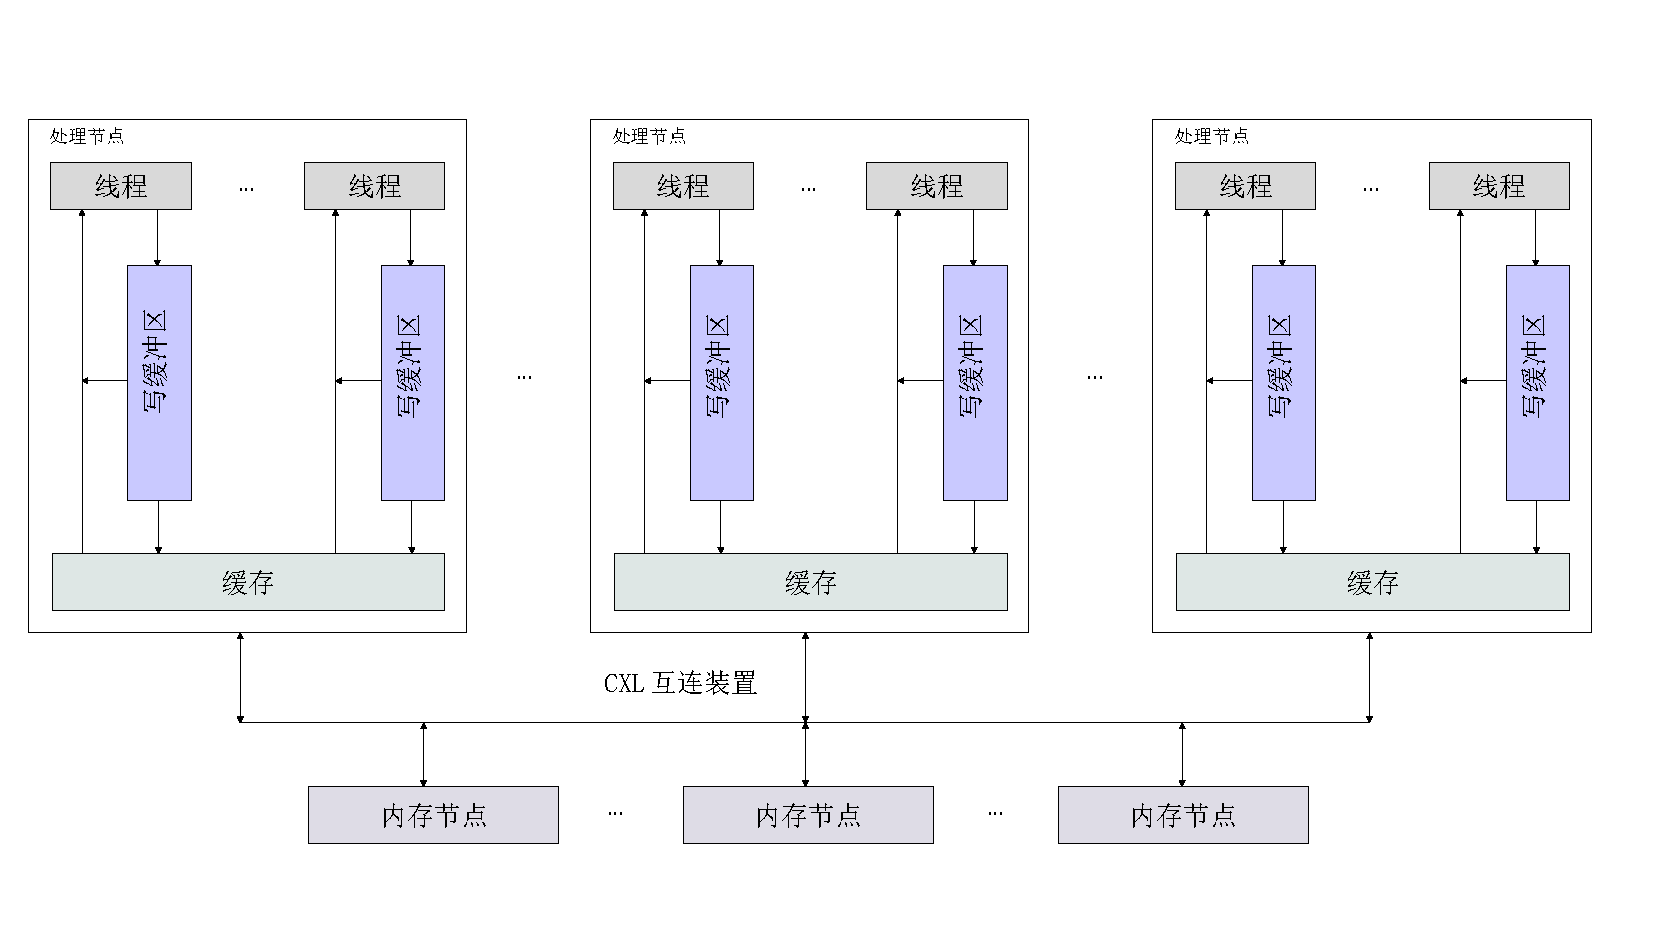
\includegraphics[width=\linewidth]{pic/cxl.pdf}
            \end{figure}
        \end{column}
    \end{columns}

    \begin{itemize}
        \item 节点：崩溃的最小单元
        \begin{itemize}
            \item 处理节点：代表一台机器，运行若干线程
            \item 内存节点：包含若干共享变量的地址
        \end{itemize}
    \end{itemize}
\end{frame}

\begin{frame}{语义框架}
    内存模型的刻画方法主要有两种：
    \begin{itemize}
        \item 操作语义：通过\highlight{变迁系统}模拟实际的内存层级行为
        \item 声明语义：通过\highlight{执行图}上的公理约束访存操作的序关系
    \end{itemize}
\end{frame}

\begin{frame}{TSO}
    % MARKER
\end{frame}

\begin{frame}{操作语义}
    \begin{definition}[标记变迁系统]
    	\label{def:lts}
    	标记变迁系统是一个五元组 $S = (Q, \Sigma, Q_0, T, \Omega)$，其中 $Q$ 是状态集合，$\Sigma$ 是由\emph{标记}构成的有限字母表，$Q_0 \subseteq Q$ 是初始状态集合，$T \subseteq Q \times \Sigma \times Q$ 是带标记的变迁集合，而 $\Omega \subseteq Q \times 2^{\nodeset} \times Q$ 是表示崩溃的变迁集合。
    \end{definition}
\end{frame}


\begin{frame}{Why Beamer}
    \begin{itemize}
        \item \LaTeX 广泛用于学术界，期刊会议论文模板
    \end{itemize}
    \begin{table}[h]
        \centering
        \begin{tabular}{c|c}
            Microsoft\textsuperscript{\textregistered}  Word & \LaTeX \\
            \hline
            文字处理工具 & 专业排版软件 \\
            容易上手，简单直观 & 容易上手 \\
            所见即所得 & 所见即所想，所想即所得 \\
            高级功能不易掌握 & 进阶难，但一般用不到 \\
            处理长文档需要丰富经验 & 和短文档处理基本无异 \\
            花费大量时间调格式 & 无需担心格式，专心作者内容 \\
            公式排版差强人意 & 尤其擅长公式排版 \\
            二进制格式，兼容性差 & 文本文件，易读、稳定 \\
            付费商业许可 & 自由免费使用 \\
        \end{tabular}
    \end{table}
\end{frame}

\begin{frame}{排版举例}
    \begin{exampleblock}{无编号公式} % 加 * 
        \begin{equation*}
            J(\theta) = \mathbb{E}_{\pi_\theta}[G_t] = \sum_{s\in\mathcal{S}} d^\pi (s)V^\pi(s)=\sum_{s\in\mathcal{S}} d^\pi(s)\sum_{a\in\mathcal{A}}\pi_\theta(a|s)Q^\pi(s,a)
        \end{equation*}
    \end{exampleblock}
    \begin{exampleblock}{多行多列公式\footnote{如果公式中有文字出现，请用 $\backslash$mathrm\{\} 或者 $\backslash$text\{\} 包含，不然就会变成 $clip$，在公式里看起来比 $\mathrm{clip}$ 丑非常多。}}
        % 使用 & 分隔
        \begin{align}
            Q_\mathrm{target}&=r+\gamma Q^\pi(s^\prime, \pi_\theta(s^\prime)+\epsilon)\\
            \epsilon&\sim\mathrm{clip}(\mathcal{N}(0, \sigma), -c, c)\nonumber
        \end{align}
    \end{exampleblock}
\end{frame}

\begin{frame}
    \begin{exampleblock}{编号多行公式}
        % Taken from Mathmode.tex
        \begin{multline}
            A=\lim_{n\rightarrow\infty}\Delta x\left(a^{2}+\left(a^{2}+2a\Delta x+\left(\Delta x\right)^{2}\right)\right.\label{eq:reset}\\
            +\left(a^{2}+2\cdot2a\Delta x+2^{2}\left(\Delta x\right)^{2}\right)\\
            +\left(a^{2}+2\cdot3a\Delta x+3^{2}\left(\Delta x\right)^{2}\right)\\
            +\ldots\\
            \left.+\left(a^{2}+2\cdot(n-1)a\Delta x+(n-1)^{2}\left(\Delta x\right)^{2}\right)\right)\\
            =\frac{1}{3}\left(b^{3}-a^{3}\right)
        \end{multline}
    \end{exampleblock}
\end{frame}

\begin{frame}{图形与分栏}
    % From thuthesis user guide.
    \begin{minipage}[c]{0.3\linewidth}
        \psset{unit=0.8cm}
        \begin{pspicture}(-1.75,-3)(3.25,4)
            \psline[linewidth=0.25pt](0,0)(0,4)
            \rput[tl]{0}(0.2,2){$\vec e_z$}
            \rput[tr]{0}(-0.9,1.4){$\vec e$}
            \rput[tl]{0}(2.8,-1.1){$\vec C_{ptm{ext}}$}
            \rput[br]{0}(-0.3,2.1){$\theta$}
            \rput{25}(0,0){%
            \psframe[fillstyle=solid,fillcolor=lightgray,linewidth=.8pt](-0.1,-3.2)(0.1,0)}
            \rput{25}(0,0){%
            \psellipse[fillstyle=solid,fillcolor=yellow,linewidth=3pt](0,0)(1.5,0.5)}
            \rput{25}(0,0){%
            \psframe[fillstyle=solid,fillcolor=lightgray,linewidth=.8pt](-0.1,0)(0.1,3.2)}
            \rput{25}(0,0){\psline[linecolor=red,linewidth=1.5pt]{->}(0,0)(0.,2)}
%           \psRotation{0}(0,3.5){$\dot\phi$}
%           \psRotation{25}(-1.2,2.6){$\dot\psi$}
            \psline[linecolor=red,linewidth=1.25pt]{->}(0,0)(0,2)
            \psline[linecolor=red,linewidth=1.25pt]{->}(0,0)(3,-1)
            \psline[linecolor=red,linewidth=1.25pt]{->}(0,0)(2.85,-0.95)
            \psarc{->}{2.1}{90}{112.5}
            \rput[bl](.1,.01){C}
        \end{pspicture}
    \end{minipage}\hspace{1cm}
    \begin{minipage}{0.5\linewidth}
        \medskip
        %\hspace{2cm}
        \begin{figure}[h]
            \centering
            \includegraphics[height=.4\textheight]{pic/dtmf.pdf}
        \end{figure}
    \end{minipage}
\end{frame}

\begin{frame}[fragile]{\LaTeX{} 常用命令}
    \begin{exampleblock}{命令}
        \centering
        \footnotesize
        \begin{tabular}{llll}
            \cmd{chapter} & \cmd{section} & \cmd{subsection} & \cmd{paragraph} \\
            章 & 节 & 小节 & 带题头段落 \\\hline
            \cmd{centering} & \cmd{emph} & \cmd{verb} & \cmd{url} \\
            居中对齐 & 强调 & 原样输出 & 超链接 \\\hline
            \cmd{footnote} & \cmd{item} & \cmd{caption} & \cmd{includegraphics} \\
            脚注 & 列表条目 & 标题 & 插入图片 \\\hline
            \cmd{label} & \cmd{cite} & \cmd{ref} \\
            标号 & 引用参考文献 & 引用图表公式等\\\hline
        \end{tabular}
    \end{exampleblock}
    \begin{exampleblock}{环境}
        \centering
        \footnotesize
        \begin{tabular}{lll}
            \env{table} & \env{figure} & \env{equation}\\
            表格 & 图片 & 公式 \\\hline
            \env{itemize} & \env{enumerate} & \env{description}\\
            无编号列表 & 编号列表 & 描述 \\\hline
        \end{tabular}
    \end{exampleblock}
\end{frame}

\begin{frame}[fragile]{\LaTeX{} 环境命令举例}
    \begin{minipage}{0.5\linewidth}
\begin{lstlisting}[language=TeX]
\begin{itemize}
  \item A \item B
  \item C
  \begin{itemize}
    \item C-1
  \end{itemize}
\end{itemize}
\end{lstlisting}
    \end{minipage}\hspace{1cm}
    \begin{minipage}{0.3\linewidth}
        \begin{itemize}
            \item A
            \item B
            \item C
            \begin{itemize}
                \item C-1
            \end{itemize}
        \end{itemize}
    \end{minipage}
    \medskip
    \pause
    \begin{minipage}{0.5\linewidth}
\begin{lstlisting}[language=TeX]
\begin{enumerate}
  \item 巨佬 \item 大佬
  \item 萌新
  \begin{itemize}
    \item[n+e] 瑟瑟发抖
  \end{itemize}
\end{enumerate}
\end{lstlisting}
    \end{minipage}\hspace{1cm}
    \begin{minipage}{0.3\linewidth}
        \begin{enumerate}
            \item 巨佬
            \item 大佬
            \item 萌新
            \begin{itemize}
                \item[n+e] 瑟瑟发抖
            \end{itemize}
        \end{enumerate}
    \end{minipage}
\end{frame}

\begin{frame}[fragile]{\LaTeX{} 数学公式}
    \begin{columns}
        \begin{column}{.55\textwidth}
\begin{lstlisting}[language=TeX]
$V = \frac{4}{3}\pi r^3$

\[
  V = \frac{4}{3}\pi r^3
\]

\begin{equation}
  \label{eq:vsphere}
  V = \frac{4}{3}\pi r^3
\end{equation}
\end{lstlisting}
        \end{column}
        \begin{column}{.4\textwidth}
            $V = \frac{4}{3}\pi r^3$
            \[
                V = \frac{4}{3}\pi r^3
            \]
            \begin{equation}
                \label{eq:vsphere}
                V = \frac{4}{3}\pi r^3
            \end{equation}
        \end{column}
    \end{columns}
    \begin{itemize}
        \item 更多内容请看 \href{https://zh.wikipedia.org/wiki/Help:数学公式}{\color{purple}{这里}}
    \end{itemize}
\end{frame}

\begin{frame}[fragile]
    \begin{columns}
        \column{.6\textwidth}
\begin{lstlisting}[language=TeX]
    \begin{table}[htbp]
      \caption{编号与含义}
      \label{tab:number}
      \centering
      \begin{tabular}{cl}
        \toprule
        编号 & 含义 \\
        \midrule
        1 & 4.0 \\
        2 & 3.7 \\
        \bottomrule
      \end{tabular}
    \end{table}
    公式~(\ref{eq:vsphere}) 的
    编号与含义请参见
    表~\ref{tab:number}。
\end{lstlisting}
        \column{.4\textwidth}
        \begin{table}[htpb]
            \centering
            \caption{编号与含义}
            \label{tab:number}
            \begin{tabular}{cl}\toprule
                编号 & 含义 \\\midrule
                1 & 4.0\\
                2 & 3.7\\\bottomrule
            \end{tabular}
        \end{table}
        \normalsize 公式~(\ref{eq:vsphere})的编号与含义请参见表~\ref{tab:number}。
    \end{columns}
\end{frame}

\begin{frame}{作图}
    \begin{itemize}
        \item 矢量图 eps, ps, pdf
        \begin{itemize}
            \item METAPOST, pstricks, pgf $\ldots$
            \item Xfig, Dia, Visio, Inkscape $\ldots$
            \item Matlab / Excel 等保存为 pdf
        \end{itemize}
        \item 标量图 png, jpg, tiff $\ldots$
        \begin{itemize}
            \item 提高清晰度，避免发虚
            \item 应尽量避免使用
        \end{itemize}
    \end{itemize}
    \begin{figure}[htpb]
        \centering
        \includegraphics[width=0.2\linewidth]{pic/Tsinghua_University_Logo.eps}
        \caption{这个校徽就是矢量图}
    \end{figure}
\end{frame}

\section{基于鲁棒性检查的验证方法}

\section{基于不变式综合的验证方法}

\section{总结与展望}

\begin{frame}
    \begin{itemize}
        \item 一月：完成文献调研
        \item 二月：复现并评测各种Beamer主题美观程度
        \item 三、四月：美化THU Beamer主题
        \item 五月：论文撰写
    \end{itemize}
\end{frame}


% \section{参考文献}

% \begin{frame}[allowframebreaks]
%     \bibliography{ref}
%     \bibliographystyle{alpha}
%     % 如果参考文献太多的话，可以像下面这样调整字体：
%     % \tiny\bibliographystyle{alpha}
% \end{frame}

\begin{frame}
    \begin{center}
        {\Huge\calligra Thanks!}
    \end{center}
\end{frame}

\end{document}
